\begin{frame}{History}
\begin{itemize}
	\item 45 year male h/o pain and difficulty walking x 2 years
	\item Difficulty in getting up from sitting position
	\item Waddling gait 
    \begin{itemize}	
		\item H/o pathological fracture bilateral neck of femur
        \item Treated elsewhere with teriparatide
    \end{itemize}
\end{itemize}
\end{frame}
%%%%%%%%%%%%%%%%%%%%%%%%%%%%%%%%%%%%%%%%%5

\begin{frame}{History}
\begin{itemize}
	\item No h/o chronic drug intake
	\item No family history of similar illness
	\item No dental abnormalities or h/o fractures in childhood
    \item No bony deformities
\end{itemize}
\end{frame}
%%%%%%%%%%%%%%%%%%%%%%%%%%%%%%%%%%%%%%%%%%
%%%%%%%%%%%%%%%%%%%%%%%%%%%%%%%%%%%%%%%%%
\begin{frame}{Biochemical parameters-Baseline}
\begin{center}
		\begin{tabular}{p{4cm}p{3.5cm}l}
			\toprule
			Parameter  & Baseline         & Reference \\ \midrule
			Calcium    & 9.2 mg/dl        & 9-11      \\
			Phosphate  & \myred{1.3 mg/dl}  & 2.5-4.5   \\
			ALP        & 146 IU/L         & 40-150    \\
			PTH        & 50.1 pg/ml       & 9 - 52    \\
			25(OH)D    & \myred{21.3 ng/ml} & 30-100    \\
			Creatinine & 1 mg/dl          & 0.8 -1.5  \\ \bottomrule
		\end{tabular} 
\end{center}
\end{frame}
%%%%%%%%%%%%%%%%%%%%%%%%%%%%%%%%%
\begin{frame}{What's going on?  }
\begin{itemize}
	\item \st{Oral intake}\footfullcite{Amanzadeh.2006}
	\item \st{Redistribution}
	\item Increased excretion
\end{itemize}
\end{frame} 
%---------------------------------------------------------------------------------- 
\begin{frame}{How to check for urinary excretion of $ PO_{4} $ ? }
	\begin{itemize}
		\item Fasting urine and serum phosphate
		\item Fasting urine and serum creatinine
		\item Calculate TmP/GFR
	\end{itemize}
\end{frame} 
%---------------------------------------------------------------------------------- 
\begin{frame}{How to calculate TmP/GFR ? }
		\begin{center}
			\begin{figure}
				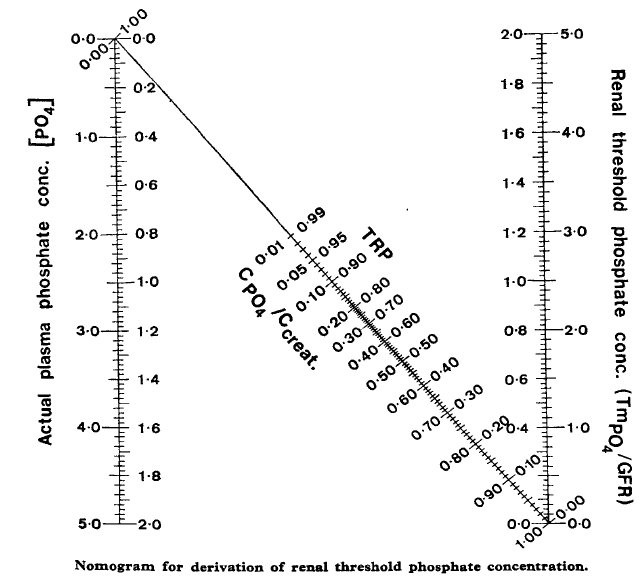
\includegraphics[scale=0.4]{nomogram.png}
				\caption{Walton and Bijvoet nomogram}
			\end{figure}
		\end{center}
\end{frame} 
%----------------------------------------------------------------------------------
\begin{frame}{How to calculate TmP/GFR?  }
	Step 1 - Calculate TRP
	\begin{block}{TRP}
		\begin{equation}
		1-\dfrac{Urine _{P}}{Urine _{Cr}} / \dfrac{Serum _{P}}{Serum _{Cr}}
		\end{equation}
	\end{block}
 Step 2 Calculate TmP/GFR
 \begin{block}{TmP/GFR}
 	\begin{equation}
 		TmP/GFR =TRP \times Serum _{P}  
 	\end{equation}
 	If TRP $ > 0.86 $
 	\begin{equation}
 	TmP/GFR =[0.3 \times TRP/(1- (0.8 \times TRP))] \times Serum _{P}
 	\end{equation}
 \end{block}
\end{frame}  
%----------------------------------------------------------------------------------
\begin{frame}{Calculating TmP/GFR  }
	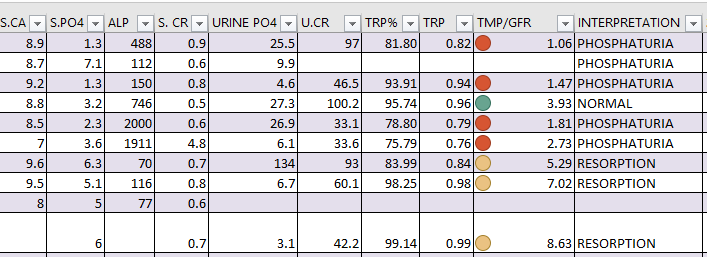
\includegraphics[width=\textwidth]{excel.png}
\end{frame}  
%---------------------------------------------------------------------------------- 
\begin{frame} {Urinalysis}
\begin{center}
		\begin{tabular}{p{4cm}p{3.5cm}l}
			\toprule
			Parameter   & Baseline  & Reference \\ \midrule
			pH          & 6.5       & 4.8 -8    \\
			Glucose     & 4+        & Nil       \\
			Aminoacids  & Positive  & Variable  \\
			Ca/Cr ratio & 0.12      & $<$ 0.2   \\
			TMP/GFR     & \myred{1.3} & 2.5-4.2   \\ \bottomrule
		\end{tabular}
\end{center}
\end{frame}
%%%%%%%%%%%%%%%%%%%%%%%%%%%%%%%%%
%---------------------------------------------------------------------------------- 


%%%%%%%%%%%%%%%%%%%%%%%%%%%%%%%%%
\begin{frame} {Bone Scan}
\begin{center}
\begin{figure}
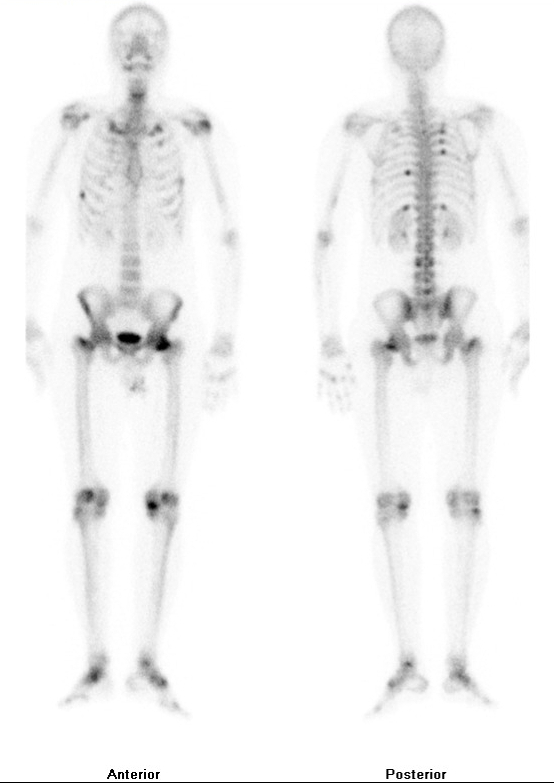
\includegraphics[height=0.7\textheight]{wholebody}
    \caption{\tiny Multiple Pseudofractures}
\end{figure}	
\end{center}	
\end{frame}
%%%%%%%%%%%%%%%%%%%%%%%%%%%%%%%%%
\begin{frame} {Description}
	\begin{itemize}
		\item Hypophosphatemic osteomalacia
        \item Proximal tubular dysfunction
\end{itemize} 
\hspace{10pt} $\oint$ Under evaluation \ldots
\end{frame}


%%%%%%%%%%%%%%%%%%%%%%%%%%%%%%%%%
\begin{frame}{Differential Diagnosis\footfullcite{Imel.2012}}
	\begin{center}
		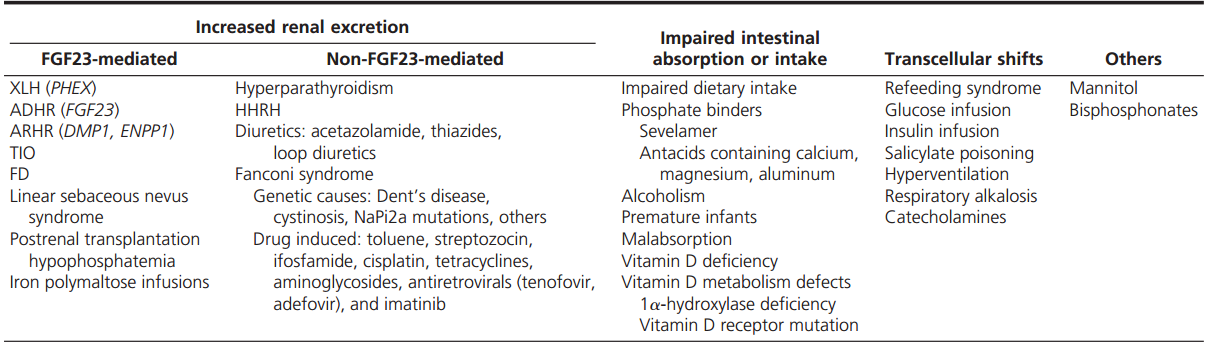
\includegraphics[width =\textwidth]{hypophosphatemia.png}
\end{center}
\end{frame}
%%%%%%%%%%%%%%%%%%%%%%%%%%%%%%%%%%%%%%%%%%%%%%%%%%%%%%%%%%
\begin{frame}{FGF23}
	\begin{block}{\textbf{C-Terminal FGF23}}
		256.7 RU/ml  (Normal: 0-150 RU/ml) 
\end{block}
\medskip\begin{bclogo} [logo=\bcbombe,barre=none,noborder=true]{Remember}
	\begin{gbar} {teal}
		FGF 23 should not be sent in serum as it gets degraded.\footfullcite{Bacchetta.2012} \\
		$ \therefore FGF \ 23 \ assay \implies EDTA \ sample $
	\end{gbar}
\end{bclogo}

\end{frame}


%%%%%%%%%%%%%%%%%%%%%%%%%%%%%%%%%%%%%%%%%%%%%%%%%%%%%%%%%%%%

%%%%%%%%%%%%%%%%%%%%%%%%%%%%%%%%%%%%%%%%%%%%%%%%%%%%%%%%%%%%%%%%%
\begin{frame}{ Interpretation }
\begin{tcolorbox}[colback=teal!5!white,colframe=teal!75!black,sidebyside]
	\begin{itemize}
	\item Hypophosphatemia
	\item Phosphaturia
	\item Normal PTH
	\item Suppressed Calcitriol
	\item High FGF 23
	\end{itemize}
	\tcblower%-----------------------------------------
	\begin{itemize}
		\item Adult onset
		\item No family history
	\end{itemize}
\end{tcolorbox}
\pause
\bigskip
$ \Longrightarrow $ TIO Vs ADHR
\end{frame} 

%---------------------------------------------------------------------------------- 
\begin{frame} {History \& Examination Revisited}
	Subcutaneous nodule of size 1.5 cm in the medial aspect of left thigh
\end{frame}

%%%%%%%%%%%%%%%%%%%%%%%%%%%%%%%%%%%%%%%%%%%%%%%%%%%%%%%%%%%%%%%%%%
\begin{frame} {Wholebody blood pool imaging}
\begin{center}
	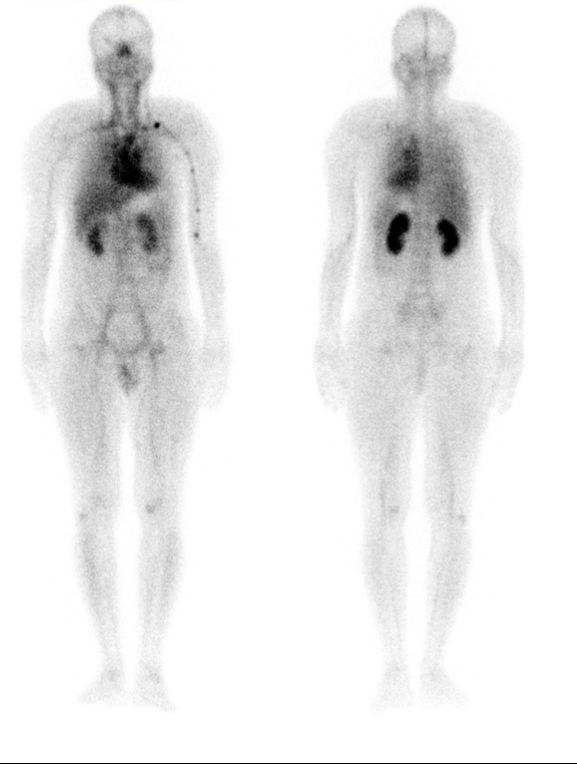
\includegraphics[scale=0.3]{bloodpool}
\end{center}
\end{frame}
%---------------------------------------------------------------------------------- 
\begin{frame}{Imaging}
	\begin{figure}
		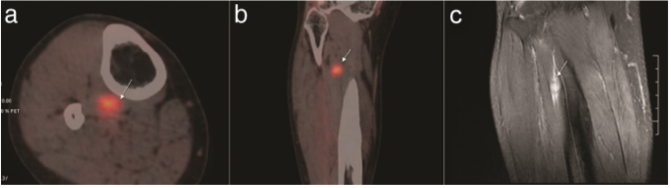
\includegraphics[scale=0.5]{fig1jcem}
       \scriptsize \caption{\textbf{a}- Fused PET-CT axial images showing FDG-avid soft tissue lesion posterolateral right proximal tibia.\\ \textbf{ b} -Fused PET-CT sagittal image of right leg showing same lesion seen on coronal section.\\ \textbf{ c} - T2 magnetic resonance coronal view shows hyperintense signal intensity right leg-SUV max : 4.86 gms/ml}
\end{figure}
\end{frame}
%%%%%%%%%%%%%%%%%%%%%%%%%%%%%%%%%%%%%%%%%%%%%%%%%%%%%%%%%%%%%%%%%%
\begin{frame}{Imaging}
\begin{center}
\begin{figure}
	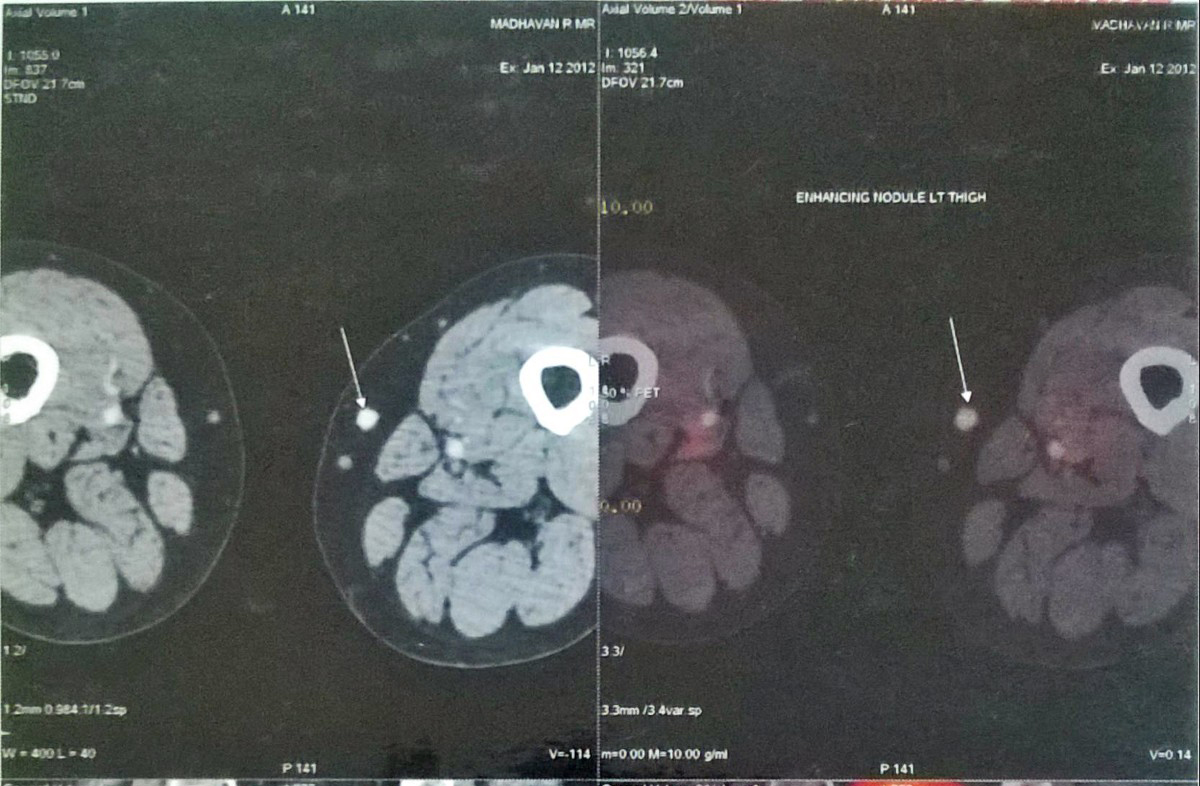
\includegraphics[scale=0.3]{thighcs}
    \caption{CT Left thigh}
\end{figure}	
\end{center}
\end{frame}
%%%%%%%%%%%%%%%%%%%%%%%%%%%%%%%%%%%%%%%%%%%%%%%%%%%%%%%%%%55%%%%5%
\begin{frame}{Imaging}
\begin{center}
\begin{figure}
	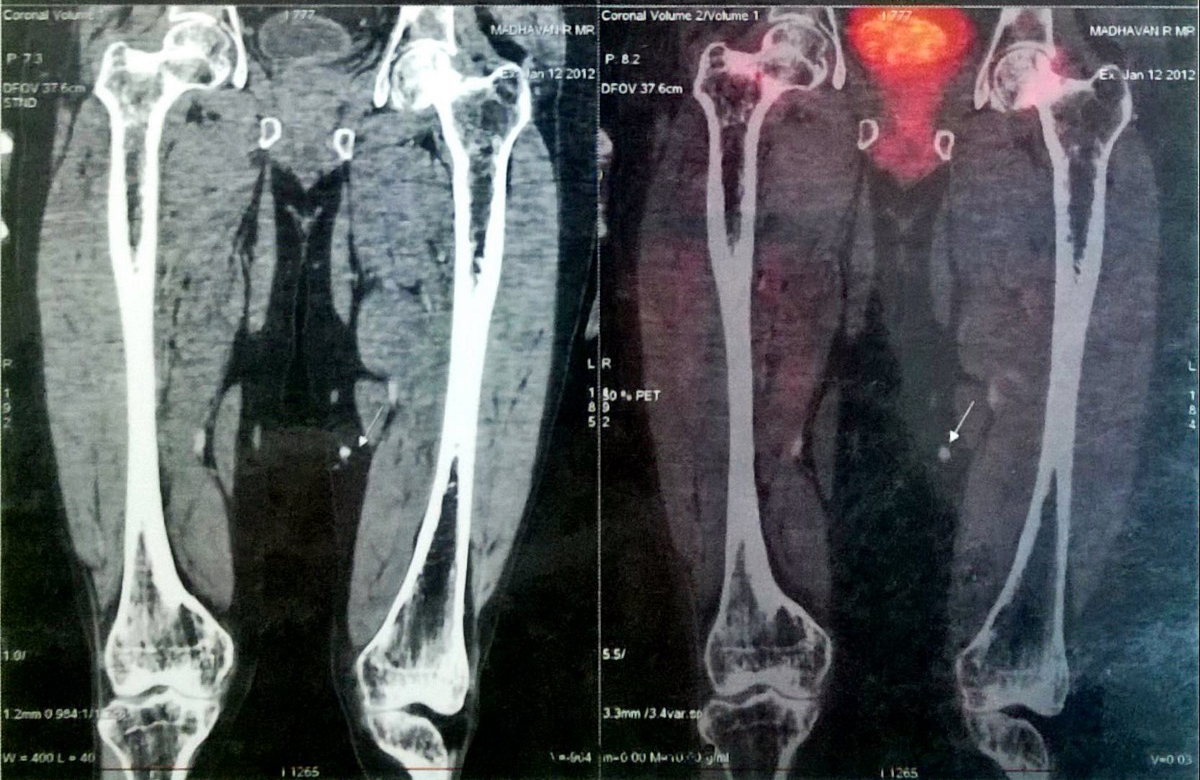
\includegraphics[scale=0.3]{thighfunc}
    \caption{PET CT(fused) Left thigh}
\end{figure}	
\end{center}
\end{frame}
%---------------------------------------------------------------------------------- 
\begin{frame}{ Imaging options \footfullcite{Jadhav.2014} }
	\begin{itemize}
		\item FDG-PET CT
		\item $ ^{99}Tc- $HYNIC-TOC SPECT CT
		\item $ ^{68} $ Ga DOTATATE 
	\end{itemize}
\end{frame}
%----------------------------------------------------------------------------------
\begin{frame}{What do we want to know?  }
\begin{block}{Conditional Probability}
  \begin{equation}
  		P(OtherScan+ | FDG -) = \dfrac{P(OtherScan+ve) \cap  P(FDG+)}{P(FDG+)}
  \end{equation}
\end{block}
\end{frame} 
%----------------------------------------------------------------------------------  
\begin{frame}{What would you do?  }
	\begin{enumerate}
         \item Remove the FDG avid lesion
         \item Remove the non FDG avid lesion
         \item Remove both
         \item Do some other scan
	\end{enumerate}
\end{frame} 

%%%%%%%%%%%%%%%%%%%%%%%%%%%%%%%%%%%%%%%%%%%%%%%%%%%%%%%%%%%%%%%%%%%%

\begin{frame}{Course}
	\begin{itemize}
		\item Patient underwent surgical excision of FDG avid lesion in the posterolateral region of right leg
        \item Post operative biochemical evaluation done
\end{itemize}
\end{frame}
%%%%%%%%%%%%%%%%%%%%%%%%%%%%%%%%%%%%%%%%%%%%%%%%%%%%%%%%%%%%%%%%%%
\begin{frame}{Biochemical parameters-Post surgery}
\begin{center}
		\begin{tabular}{p{4cm}p{3.5cm}}
			\toprule
			Parameter                 & Post Surgery \\ 
            \midrule
			Calcium                   &  7.7 mg/dl \\
			Phosphate                 & \myred{1.2 mg/dl}\\
			ALP                       & 105 IU/L \\
            TMP/GFR                   & 1.5       \\   
			\textbf{C-Terminal FGF23} & \myred{102 RU/ml}  \\
			 \bottomrule

		\end{tabular} 
\end{center}
\end{frame}
%%%%%%%%%%%%%%%%%%%%%%%%%%%%%%%%%%%%%%%%%%%%%%%%%%%%%%%%%%55%%%%5%
\begin{frame}[plain]{Histopathology}
 \begin{figure}
	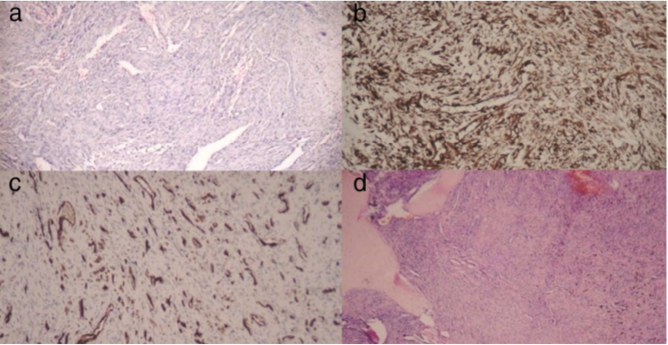
\includegraphics[scale=0.45]{fig2jcem}
    \tiny{
    	\caption{A, Proliferation of spindle cells in small fascicles and the striking
hemangiopericytomatous pattern. B, Positivity of the tumor cells for
vimentin. C, CD 34 highlighting the blood vessels and thus the
hemangiopericytomatous pattern. D, Tumor composed of spindle cells and
metaplastic osteoid formation along with focal areas showing hemosiderin-laden macrophages}
}
\end{figure}
\end{frame}
%%%%%%%%%%%%%%%%%%%%%%%%%%%%%%%%%%%%%%%%%%%%%%%%%%%%%%%%%%%%%%%%%%
\begin{frame} {Course\ldots}
	\begin{itemize}
		\item Failed first surgery in spite of complete tumor excision
        \item Waited for 8 weeks to rule out delayed remission
        \item Underwent removal of FDG negative lesion in left medial thigh
\end{itemize}
\end{frame}



%%%%%%%%%%%%%%%%%%%%%%%%%%%%%%%%%%%%%%%%%%%%%%%%%%%%%%%%%%%%%%%%%
%%%%%%%%%%%%%%%%%%%%%%%%%%%%%%%%%%%%%%%%%%%%%%%%%%%%%%%%%%%%%%%%%%
\begin{frame}{Biochemical parameters-Post surgery}
\begin{center}
		\begin{tabular}{p{4cm}p{3.5cm}l}
			\toprule
			Parameter                 & Post Surgery-1             & Post Surgery-2      \\ 
            \midrule
			Calcium                   &  7.7 mg/dl            & 9.3 mg/dl          \\
			Phosphate                 & 1.2 mg/dl            & 4.3 mg/dl        \\
			ALP                       & 105 IU/L             & 162 IU/L         \\
            TMP/GFR                   & 1.5                  & 2.4   \\   
			\textbf{C-Terminal FGF23} & \textbf{102 RU/ml} & \textbf{22 RU/ml} \\
			 \bottomrule

		\end{tabular} 
\end{center}
\end{frame}
%%%%%%%%%%%%%%%%%%%%%%%%%%%%%%%%%%%%%%%%%%%%%%%%%%%%%%%%%%%%%%%%%%
\begin{frame} {Final Diagnosis}
	\center Tumor(s) Induced Osteomalacia \footfullcite{Sahoo.2014}
\end{frame}
%%%%%%%%%%%%%%%%%%%%%%%%%%%%%%%%%%%%%%%%%%%%%%%%%%%%%%%%%%%%%%%%%%


